% !TEX root = ../../report.tex

\section{Original Assignment Text}\label{intro:original-text}

\paragraph{Task: Construct a Multiple Instruction, Multiple Data Processor}
The performance increase available from harvesting Instruction Level Parallelism
(ILP) from the serial instruction stream is limited because we have reached the
maximum power consumption that can be handled without expensive cooling
solutions\cite{olukotun}. Consequently, there is a significant interest in
single-chip parallel processor solutions (e.g. \cite{bell,kongetira}). The
processor cores in commercial multi-core chips are conventional designs and
therefore reasonably complex. In this work, your task is to design a
multiprocessor, Multiple Instruction, Multiple Data streams (MIMD). A processor
classified MIMD include a multiple- instruction stream
organizations\cite{flynn}. Such processors can executing different instructions,
i.e. minimum 2 independent programs, on different (independent) data.

The task also include that a suitable application is chosen to demonstrate the
processor. Your processor will be implemented on an FPGA, and you are free to
choose how to realize your MIMD computer architecture. The system should be
shown to work with a suitable application. Studying the architecture of the
Cell processor\cite{wiki_cell_mpu}, or in general multi-core
processors\cite{wiki_multicore}, can be a good starting point. And a final tip;
Keep it simple, as simple as possible, but not simpler. Due to a large number of
students this year, we will divide the work into two independent projects: a)
Performance and b) Energy efficiency. The goal of group a) is to achieve maximum
performance while group b) should try to balance performance and energy. The
reports from both groups should include an evaluation of prototype performance
and energy consumption.

\paragraph{Additional Requirements}
The unit must utilize a Silicon Labs microcontroller and a Xilinx FPGA. The
budget is 10.000 NOK, which must cover components and PCB production. The unit
design must adhere to the limits set by the course staff at any given time.
Deadlines are given in a separate time schedule.

\paragraph{Evaluation}
The project is evaluated based on the project report and an oral presentation of
the work as well as a prototype demonstration. One grade will be given to the
group as a whole, unless there are significant variations in the amount of
effort put into the project.

\section{Assignment}

\paragraph{Assignment Interpretation}\label{intro:our-assignment-interpretation}
Our interpretation of the assignment is to design a hardware prototype system for a
specific application domain with two main components. First, it must have a
\textit{microcontroller} (MCU). Second, it must have a \textit{Field Programmable Gate Array} (FPGA)
implementing a MIMD architecture processor. The project design must fit on a custom
made \textit{Printed Circuit Board} (PCB) developed for this project. On behalf of these
requirements, this results in a convenient division of labour where the MCU manages
the peripherals and drives the system, while the FPGA is being used as a hardware
accelerator, i.e. to speed up execution of programs.

Another design requirement given from the assignment description is energy
efficiency. The hardware configuration with a general processor and a
specialized set of processors has become increasingly popular since power
consumption became an issue, and is ubiquitous in today's computing systems.
Being on the energy efficiency group motivates us to leverage such energy aware
concepts and design a system with energy efficiency in mind.

\missingfigure{A figure giving a ``20k feet view from above'' of the PCB, MCU,
and FPGA.}
\begin{figure}[H]
    \centering
    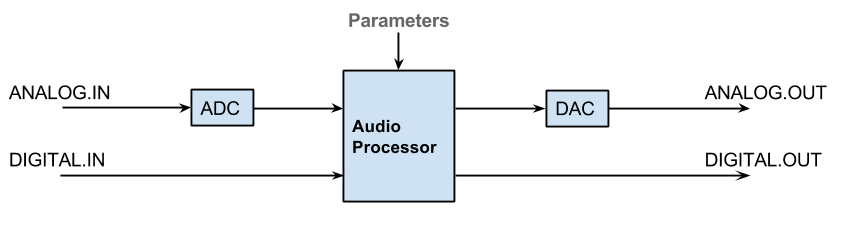
\includegraphics[height=150px]{figures/intro/intro_audio_analog_digital.png}
    \caption{An abstract view of the two audio processiong options.}
    \label{fig:audio_path_overview}
\end{figure}


The above \todo{Insert reference}figure shows how the FPGA processor
design can run different programs with a MIMD architecture.

The application chosen for this project is audio processing. The MCU will
provide audio samples from a source on the PCB to the FPGA, which in turn will
process the samples and return the result. As the FPGA contains multiple cores,
the FPGA may run different filters, transforms, and effects in parallel on the
audio samples. For the rest of this report, the Giant Gecko microcontroller unit
from Silicon Labs is hereafter referred to as the MCU, and the Spartan-6 Xilinx
FPGA chip will hereafter be referred to as the FPGA. The processor design
written in VHDL and implemented on the FPGA is hereafter referred to as
Concurrent Homogenous Audio Optimized Streaming Microprocessor (\textit{ChaosM}).

\subsection{Energy Efficiency}
Since this project belongs to the energy efficiency group of the TDT4295 course,
an important focus during the planning, implementation, and testing of this system
has been energy efficiency.

While a Xilinx Spartan-6\cite{fpga-chip} processing core does not have much
potential for energy efficiency, the aim is to program the design and simulate
energy efficiency through \textit{ChaosM} on the FPGA, as well as in the
programming on the MCU, and in the design of the PCB.

The MCU is branded as an ``energy friendly microprocessor'', with many features
which when implemented correctly can hold immense potential for energy savings
compared to most other microprocessor units on the market.

The PCBs in previous TDT4295 projects have often been the culprit at the root of
energy inefficiency. Thus, in this project there has been a lot of focus on making
the source of all the energy work as energy efficiently as possible, as well as
utilizing components in an energy efficient manner.

More details on how the different parts of the system utilizes energy efficient
implementations for this project, can be found in their respective sub-sections
of chapter \ref{chapter:implementation}.

\subsection{Multiple Instruction, Multiple Data}

As stated in the the original assignment text, part of the requirements for this
assignment is to implement a processor design on the FPGA based on a MIMD
architecture. MIMD architecture is an extension of the Single Instruction,
Multiple Data (SIMD) architecture. In a SIMD architecture, each processor core
shares instruction memory, so in effect, all the processor cores in the
processor run the same program, but on different sets of data. Like for example
in a graphics pipeline.

A MIMD architecture however differs from the SIMD in that each processor core
has its own instruction memory, with the effect that each processor core can
perform a different task, and execute it on a different set of data than any
other core.

So for this project to successfully meet the requirements, it has to implement
an architecture with multiple processing cores, where each core can work on any
set of data with any set of instructions independently of any other core.
